
\chapter{General Background and Fundamental Concepts}
\label{chapter:general-background}

This chapter presents the general background and fundamental concepts related to the domain problem that is addressed in this thesis. At the first section (\autoref{sec:cscl-and-scripted-collaboration}), an overview of the CSCL field and scripted collaboration is presented to provide a comprehensive and clear understanding about the research context. %This section also describes in detail the motivation problem caused by the scripted collaboration when CL activities are orchestrated and structured by CSCL scripts, as well as, the related works and current computer-based solutions to deal with this problem.
The \autoref{sec:gamification} elaborates an overview of gamification, and the best practices and theories related to this technology. % Furthermore, this section presents related works that use gamification in the context of CSCL and other contexts to deal with the motivation problem are presented in this section.
Finally, the \autoref{sec:ontologies-and-ontology-engineering} presents the fundamentals of ontologies and ontology engineering.% This sections also discusses how ontologies is currently used to support the systematic formalization of theory-based knowledge, and how this formalization, in the field of artificial intelligence in education, is used to overcome problems that are similar to those that must be solved to provide a computational support in the gamification of CL scenarios with theoretical justifications based on the best practices and theories related to gamification.

%%%%%%%%%%%%%%%%%%%%%%%%%%%%%%%%%%%%%%%%%%%%%%%%%%%%%%
\section{CSCL and Scripted Collaboration}
\label{sec:cscl-and-scripted-collaboration}

Although CL has a long history in education, it is not until the early 1990s that the research field dedicated to study how to provide support for the CL through the use of Internet and computational technology had gained attention and strength \cite{StahlKoschmannSuthers2006}. Such research field known as Computer-Supported Collaborative Learning (CSCL) is a multidisciplinary field that combines studies from the cognitive psychology education and from the computer science to effectively enhance the CL process through the use of computational technology \cite{HoppeOgataSoller2007}.

The general aim of CSCL field is to develop technologies to support or create situations in which two or more students learn together through the interaction among them \cite{Dillenbourg1999}. In these situations, the learning outcomes is consequence of students' interactions and how these interactions affect the individual learning for each one of the students. In consequence, to enable a well-though-out design of CL, the CSCL scripts have been proposed by the CSCL community as the technology to facilitate the social and cognitive processes of learning by describing the way in which the learners will interact with each other in a CL scenario \cite{HarrerKobbeMalzahn2007}.

\subsection{CSCL Scripts}
\label{sec:cscl-scripts}

CSCL scripts are the technology that describes how to structure and orchestrate the CL process to attain a set of pedagogical objectives defined by an instructional design \cite{DillenbourgJermann2007}. Such description is provided in the CSCL scripts through prescribed instructions that indicates how to facilitate the social and cognitive processes in group activities \cite{Dillenbourg2002}. These prescribed instructions are defined by instructors, like teachers or instructional designers, as a way to attain a set of learning goals, and they indicate the way in which students should collaborate, they constrain the interactions among the participants, they specify the roles for the participants, they indicate the distribution of task, tools, and resources used in the CL process.

In order to narrow the number of elements used to describe the CSCL scripts, and provide a common and sharable description of CSCL scripts, \citeonline{KobbeWeinbergerDillenbourgHarrerHamalainenHakkinenFischer2007} propose a framework that is currently wide accepted by the community as the common specification to describe the CSCL scripts using natural language. This framework formalizes the CSCL scripts as a set of components and mechanisms illustrate in \autoref{fig:components-and-mechanisms-of-cscl-scripts}.


\begin{figure}[htb]
 \caption{Components and mechanisms of CSCL scripts}
 \label{fig:components-and-mechanisms-of-cscl-scripts}
 \centering
 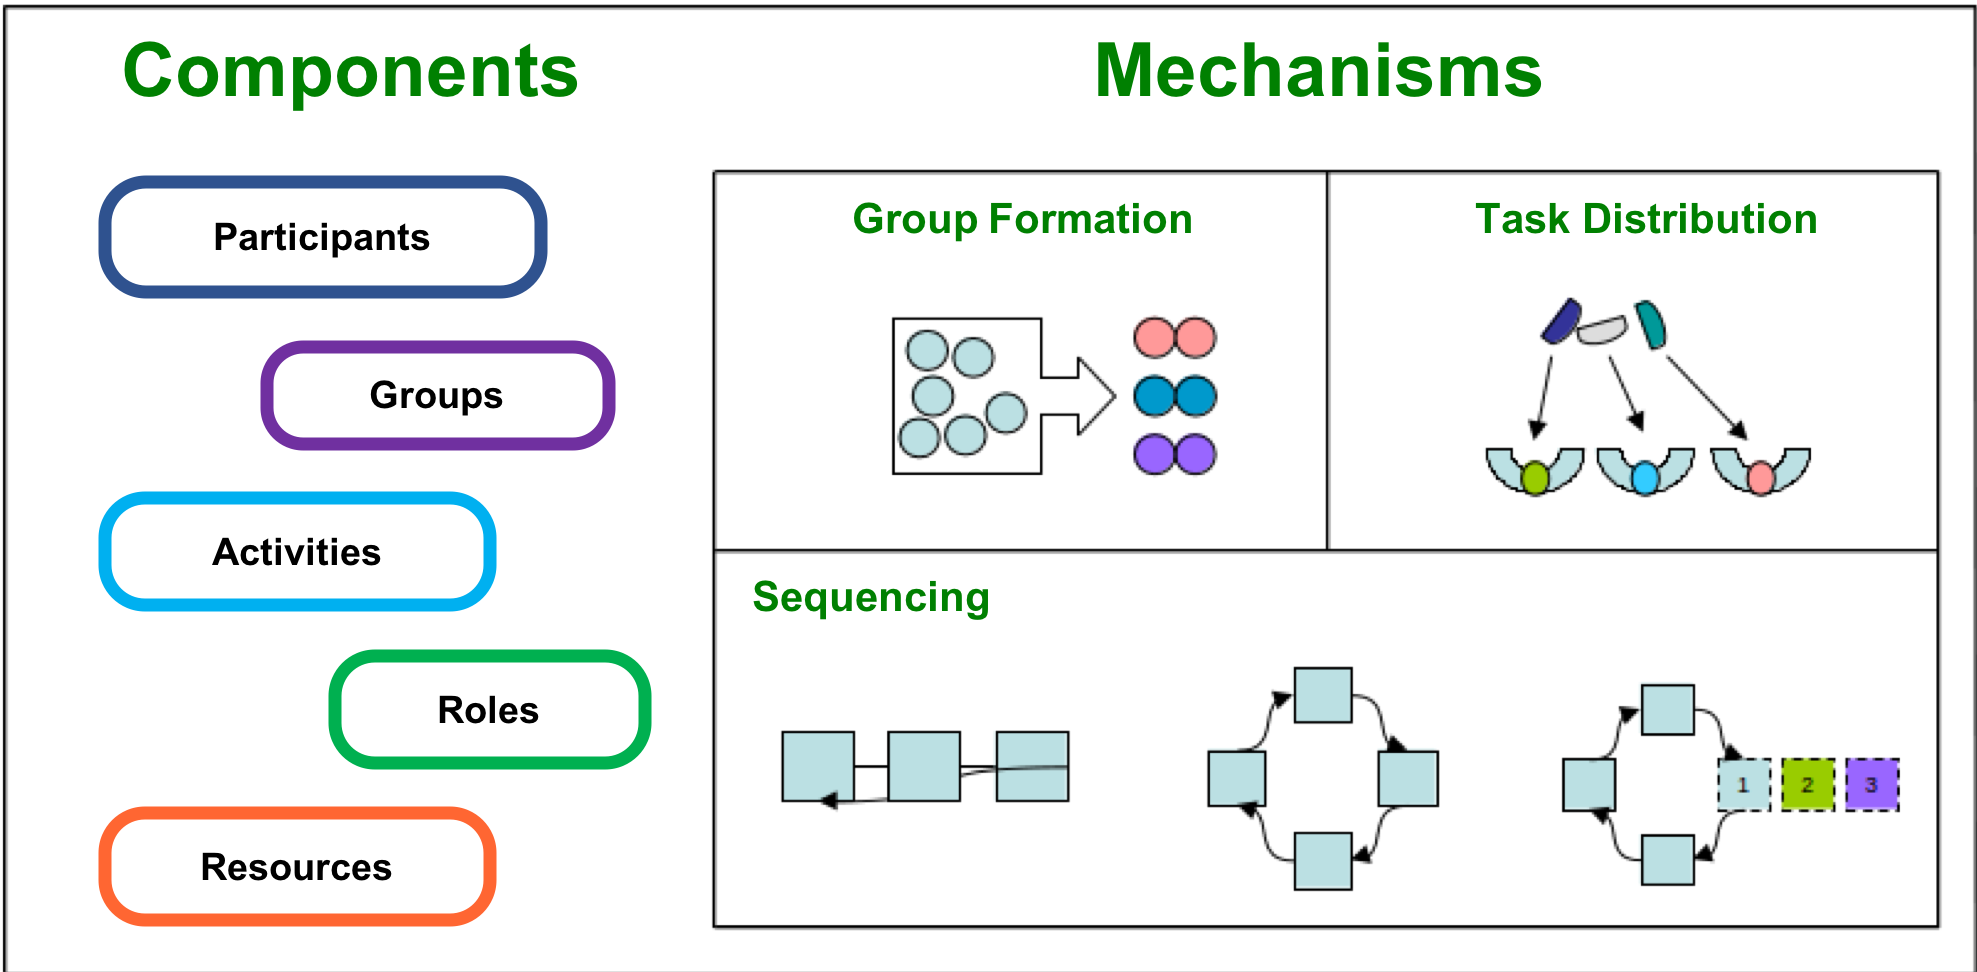
\includegraphics[width=0.95\textwidth]{images/components-and-mechanisms-of-cscl-scripts}
 \fadaptada{Fischer2007}
\end{figure}

The structural \emph{components} of CSCL scripts are the participants, groups, activities, roles and resources. The component of \emph{participants} is used to describe the participants, such as learners, monitors, and teachers. Although this description can be abstract or concrete and simple or complex, it is often presented in a simple manner with rules that indicate conditions to participate in the CL process. The component of \emph{activities} describes what will be performed by the participants in the CL process to attain the learning goals defined by the instructional designers. The component of \emph{roles} describes the privileges, obligations and expectations of participants in the CL process. The component of \emph{groups} of participants defines through hierarchical structures how the students are grouped according to the participants' characteristics. The component of \emph{resources} describes the learning objects (e.g. content, material, and tools) that can be used by the participants during the CL process.

The \emph{mechanisms} of CSCL scripts are the group formation, component distribution and sequencing. The mechanism of \emph{group formation} consists in the specifications of how the participants will be distributed over the groups. The mechanism of \emph{task distribution} provides the specification about how the components of scripts are distributed over groups using the mapping of groups, activities, roles, and resources. The mechanism of \emph{sequencing} consists in the definition of how the components and groups defined in scripts are distributed over time. In general, this sequencing describes the execution order of activities in the CL process.

\autoref{qua:social-script-framework-kobbe} shows the description of social script \cite{WeinbergerErtlFischerMandl2005} using the framework proposed by \citeonline{KobbeWeinbergerDillenbourgHarrerHamalainenHakkinenFischer2007}. In this example, the CL scenarios orchestrated by the social script foster the acquisition of knowledge through a set of case studies (\emph{resources}) that are analyzed and reviewed by the students groups. The number of students in each group is equal to the number of case studies, and the ideal number is three. In the first step of sequencing, each learner playing the \emph{analysis} role writes down an analysis of case study, and then, he critiques the analyses made by other learners playing the \emph{critics} role. In the second step of sequencing, each learner revises his/her own analysis, taking into consideration the critiques received by the other learners in the case group.

\begin{quadro}[htb]
\caption{Social script describes using the framework proposed by  \citeonline{ KobbeWeinbergerDillenbourgHarrerHamalainenHakkinenFischer2007}}
\label{qua:social-script-framework-kobbe}
\centering
\footnotesize
\begin{tabular}{l p{12cm}}
\toprule
\multicolumn{2}{l}{\textbf{Structural components:}} \\ \midrule
\textbf{Participants:} &
A number of participants that must be divisible by the number of case studies.  \\
\textbf{Groups:} &
Case groups \\
\textbf{Activities:} &
(a) Applying theoretical concepts to the case study and constructing arguments \\
 &
(b) Critiquing initially scaffolder with prompts for eliciting clarification, identifying conflicting views and constructing counter-arguments \\
\textbf{Roles:} &
\emph{Analyst} and \emph{Critic} \\
\textbf{Resources:} &
Case studies (minimal number is three case studies) \\
\toprule
\multicolumn{2}{l}{\textbf{Mechanisms}:} \\ \midrule
\textbf{Group formation:} &
All participants are grouped by the number of case studies. Each participant becomes member of all case groups although with different roles in each. Each participant is the responsible analyst for one case study and critic for all other cases \\
\textbf{Task distribution:} &
Each case group receives one case study, and the roles are distributed in a way that each participant assumes the role of analyst in one case group and the role of critic in all other case groups \\
\textbf{Sequencing:}
& - the analyst writes an analysis of case study. (a) \\
& - wait for all case group analysts to be done, and writes a critique for the analysis of case study. (b) \\
& - wait for all case group critics to be done, and the analyst considers each critique and writes a reply to each. (a) \\
& - wait for all case group analysts to be done each critic in turn reads the reply and writes a second critique. (b) \\
& - wait for all case group critics to be done... the analyst considers all critiques and revises the analysis of case study (a) \\
\bottomrule
\end{tabular}
 \fadaptada{KobbeWeinbergerDillenbourgHarrerHamalainenHakkinenFischer2007}
\end{quadro}


Having the description of CSCL scripts only in natural language does not allow the computers programs to interpret them, and to run a CL scenario following the instructions indicated by the scripts without human intervention. Therefore, to represent the CSCL scripts in a computer readable manner, the IMS-Learning Design\footnote{\url{http://www.imsglobal.org/learningdesign/}} (IMS-LD) specification has been adopted by different tools, such as (web)COLLAGE \cite{Hernandez-LeoVillasclaras-FernandezAsensio-PerezDimitriadisJorrin-AbellanRuiz-RequiesRubia-Avi2006,Villasclaras-FernandezHernandez-LeoAsensio-PerezDimitriadis2013}, CIAN \cite{MolinaRedondoOrtega2012}, LeadFlow4LD \cite{Palomino-RamirezBote-LorenzoAsensio-PerezDimitriadis2008}, NUCLEO \cite{SanchoFuentes-FernandezFernandez-Manjon2008}, CoLearn \cite{StylianakisArapiMoumoutzisChristodoulakis2013}, CeLS \cite{RonenKohen-Vacs2009}, and LAMS \cite{Romero-MorenoOrtegaTroyano2007}, as the language to describe CSCL scripts.
 
Despite the benefits that brings  the use of the IMS-LD specification to represent CSCL scripts, several researchers had indicated that this language is insufficient to fully support the modeling of CSCL scripts \cite{AlharbiAthaudaChiong2014, CaeiroAnidoLlamas2003}. Of course, the purpose of IMS-LD specification is not to provide a full support for describing CSCL scripts in a computer-readable manner, the IMS-LD has been developed as a neutral, generic and flexible educational modeling language to describe a wide range of pedagogies approaches (the teaching strategies, pedagogical goals and their associated activities) \cite{Koper2005}. In this sense, to support the representation of CSCL scripts in a computer-readable manner, a wide variety of extensions on the IMS-LD elements has been proposed in by several researchers \cite{Bote-LorenzoVaquero-GonzalezVega-GorgojoDimitriadisAsensio-PerezGomez-SanchezHernandez-Leo2004, LeoPerezDimitriadis2004, MagnisalisDemetriadis2012, MiaoHoeksemaHoppeHarrer2005, Vega-GorgojoBote-LorenzoGomez-SanchezDimitriadisAsensio-Perez2005}.

Instead, to simply provide a computer-readable representation of CSCL scripts, the work of \citeonline{Isotani2009} proposes the formalization of these scripts in a computer-understandable manner through the use of ontologies. This solution consists in a set of ontological structures that makes the description of CSCL scripts more semantically-rich, allowing the explicit specification of learning goals, purposes, and other relevant information that cannot be represented using the IMS-LD specification, i.e., learning strategies, group goals, interaction patters from learning theories. Providing this formalization in the CL ontology, \citeonline{IsotaniMizoguchiIsotaniCapeliIsotanideAlbuquerqueBittencourtJaques2013} demonstrates that intelligent-theory aware systems can interpret these scripts and provide advice and recommendation to support for the modeling of learners' development \cite{InabaIkedaMizoguchi2003}, the formation of effective groups \cite{IsotaniMizoguchi2008a}, and the instructional design of CL activities \cite{IsotaniMizoguchiIsotaniCapeliIsotanideAlbuquerqueBittencourtJaques2013}.

\subsection{Levels of Abstraction and Granularity of CSCL Scripts}
\label{sec:level-of-abstraction-and-granularity-of-cscl-scripts}

CSCL scripts have different levels of abstraction and granularity in the description of CL scenarios \cite{Dillenbourg2002, DillenbourgJermann2007, Villasclaras-FernandezIsotaniHayashiMizoguchi2009}. This classification of scripts in two dimension, abstraction and granularity, gives them an enormous flexibility to be reused in the instructional design process of CL scenarios, and it also allows the use of multiple scripts to describe different aspects of CL scenario in separated scripts. Whereas the levels of abstraction classify a script according to the completeness of elements described by them (from the most abstract to the most concrete), the levels of granularity classify the scripts according to the aggregation level of elements described by them (from the most coarser grained to the finest grained).

According to \citeonline{DillenbourgJermann2007}, a CSCL script can be classified in one of the four levels of abstraction defined as follows as:

\begin{description}
\item[\emph{Script Schemata}:] are scripts use to describe the core instructional design principles whereby is expected to trigger interactions among participants in the CL process. In this sense, these scripts are defined in a content free didactic form, so that they can be used to describe patterns of CL. Examples of script schemata are the Jigsaw script \cite{Aronson1978, KordakiSiempos2010}, conflict script \cite{WeinbergerErtlFischerMandl2005}, and reciprocal script \cite{King2007}. The jigsaw script describes a CL scenario in which the principle of interaction consists in the grouping and re-grouping of participants with complementary information to share their knowledge. The conflict script describes a CL scenario to group learners with contradictory knowledges or opinions to instigate the discussion. The reciprocal script describes a CL scenario that assigns alternate roles to the students for facilitating questioning and tutoring activities.

\item[\emph{Script Classes}:] are specialization of scripts schemata for a specific learning context. This specialization is not absolute complete, so that script classes are independent in the content-domain and student data. The script classes cover a range of scripts that describe variations of a prototype with particular details related to a specific learning context of a script schemata to facilitate its adoption. These details are, for example, the number of participants, and the king of content (matter) that will be taught. In this sense, a script class is based in a script schemata to describe CL scenarios for a specific learning context. For instance, the Universanté Script \cite{DillenbourgJermann2007} is a script class based on Jigsaw schema that was designed to describe CL scenarios for learning contexts with different thematic groups and participants from different nations.

\item[\emph{Script Instances}:] are scripts in which the content-domain are specified for a particular situation. A script instance is more concrete than a script class, and it has been instantiated from a script schema or class to be reusable more or less by teachers who only need to define participants' data. These scripts are more concrete that script classes, but they are independent in the particularities of students and learning environment.

\item[\emph{Script Sessions}:] are scripts in which the content-domain and participants data are specified to be directly executed in a learning environment. In this sense, these scripts detail the information of participants and content-domain in the most concrete level defining, for example, the students' names and the deadlines of activities. A CL scenario that is described by a script session is known as CL session, and when it is represented in a script session using a computer-readable formalization, it can be directly executed in a learning environment to orchestrate and conduct the CL process.
\end{description}

Different benefits from the use of script schemata and classes as patterns are obtained in the instructional design process of CL scenarios \cite{AlharbiAthaudaChiong2014, ChallcoBittencourtIsotani2016, MiaoHoeksemaHoppeHarrer2005}. During the design/authoring phase, repositories of script schemata and classes facilitate the sharing and reuse of these scripts in distributed learning environments \cite{PrietoAsensio-PerezMunoz-CristobalDimitriadisJorrin-AbellanGomez-Sanchez2013, PrietoTchounikineAsensio-PerezSobreiraDimitriadis2014}. The structures of script schemata and classes are used as templates to create new script schemata and classes \cite{AndreasHarrerUlrchHoppe2007, RonenKohen-Vacs2009}. 

During the instantiation/production phase, script schemata and classes provide advice and recommendation that help the CL practitioners to instantiate these scripts and to obtain CL sessions \cite{MagnisalisDemetriadis2012a, PrietoAsensio-PerezDimitriadisGomez-SanchezMunoz-Cristobal2011,Alario-HoyosBote-LorenzoGomez-SanchezAsensio-PerezVega-GorgojoRuiz-Calleja2013}. Script schemata and classes facilitate the generation of computer-interpretable scripts, they provide information to support the search of applicable learning material and tools for the CL scenario \cite{Bote-LorenzoVaquero-GonzalezVega-GorgojoDimitriadisAsensio-PerezGomez-SanchezHernandez-Leo2004, IsotaniMizoguchi2008a, Vega-GorgojoBote-LorenzoGomez-SanchezDimitriadisAsensio-Perez2005}. The script schemata and classes are also uses to obtain recommendation about how to bind individuals in groups and roles according to the knowledge described in these scripts \cite{IsotaniMizoguchiIsotaniCapeliIsotanideAlbuquerqueBittencourtJaques2013,Villasclaras-FernandezHernandez-GonzaloLeoAsensio-PerezDimitriadisMartinez-Mones2009}.

Regarding to the level of granularity \cite{FischerKollarStegmannWeckerZottmann2013}, the CSCL scripts can be classified in macro-scripts and micro-scripts.

\begin{description}
\item[\emph{Macro-scripts}:] are scripts that basically describe the CL process in a courser-grained level without detailing the specific interactions among participants. A macro-script describes how to attain a set of pedagogical objective indicating the sequencing of individual and group activities that must be follow by participants. Thus, for example, in the Jigsaw macro-script, to promotes the individual accountability and positive interdependence, the sequencing of activities consists in three activities: an individual activity, expert group activity, and jigsaw group activity. In the individual activity, each student studies a particular part of a whole problem. In the expert group, the students of different groups that study the same part of the whole problem meet together for exchanging ideas. At last activity, students of each jigsaw group meet to contribute with their expertise to solve the whole problem.

\item[\emph{Micro-scripts}:] are scripts that describe the CL process in a fine-grained level \cite{WeinbergerFischerStegmann2005}, they indicate, for example, the dialogues that must happen among student to achieve the pedagogical objectives, and they are intended to describe the communication model between participants. Thus, for example, to facilitate the negotiation and elaboration of a domain concepts, Weinberger, Ertl, Fischer, and Mandl  \cite{WeinbergerErtlFischerMandl2005} describe a micro-scripts for online peer discussion using a sequence of sentence openers (e.g. my proposal for an adjustment of the analysis is….) that prompted learners to contribute with the discussion and critique one another's contributions.
\end{description}

As can be noticed above, the macro-scripts and micro-scripts have a hierarchical relationship to describe the CL process of CL activities. The micro-scripts describe the communication process in a CL activity \cite{WeinbergerFischerStegmann2005}, whereas the macro-scripts describe groups, roles, and flow of CL activities \cite{DillenbourgHong2008}. Despite this explicit hierarchical relationship, there are few models and tools in which all the elements of macro-scripts and micro-scripts are combined to support the design of CL scenarios \cite{AlharbiAthaudaChiong2014, ChallcoBittencourtIsotani2016}. \citeonline{Hernandez-LeoVillasclaras-FernandezAsensio-PerezDimitriadisRetalis2006} propose a hierarchical model in which schemata and classes of macro-scripts and micro-scripts are used as templates to generate scripts. In the work of \citeonline{ChallcoGerosaBittencourtIsotani2014}, the hierarchical relationships of macro-scripts and micro-scripts is represented as hierarchical task networks to support the automatic generation of unit of learning.

In the CL ontology \cite{IsotaniInabaIkedaMizoguchi2009}, and therefore in the ontology OntoGaCLeS, the hierarchical relationship of macro-scripts and micro-scripts is not explicitly described as a direct link between macro- and micro-scripts. The hierarchical relationship is implicitly described as part of the conceptualization of events and processes proposed by Galton and Mizoguchi \cite{GaltonMizoguchi2009}. Based on in this conceptualization in which the representation of an event can be constituted by many distinct sub-events to describe a process, the hierarchical relationship of macro- and micro-scripts can be inferred from these events that are explicitly described in the CL ontology and the ontology OntoGaCLeS.

%%%%%%%%%%%%%%%%%%%%%%%%%%%%%%%%%%%%%%%%%%%%%%%%%%%%%%
\section{Gamification}
\label{sec:gamification}

\subsection{Gamification of Learning and Instruction}


\subsection{Flow Theory and Learning and Gamification}


%In the context of education, learners in the flow state frequently experience positive affect and better scores/performances compared with other learners who are in a similar situation but not in the flow state \cite{BaydasKarakusTopuYilmazOzturkGoktas2015, IbanezDiSerioVillaranDelgadoKloos2014, ShernoffCsikszentmihalyiSchneiderShernoff2014}. For example, several empirical studies conducted by D’Mello, Graesser, and colleagues using intelligent tutoring systems (e.g. AutoTutor) have shown strong positive correlations between learning gains, confusion, and flow state \cite{D'MelloGraesser2012}. Another example is the study of Choi et al., where participants used a web-based e-learning system in a program on Enterprise Resource Planning. The data of this study revealed that flow experiences were directly linked with learning outcomes and leaners’ attitude towards e-learning.

%According to previous findings, having an explicit formalization of the minimum and maximum difficulty/challenge levels to maintain the learners' flow is one of the key features needed to promote more effective and robust learning in different scenarios \cite{Esteban-MillatMartinez-LopezHuertas-GarciaMeseguerRodriguez-Ardura2014, FulmerD'MelloStrainGraesser2015 ,LinehanBellordKirmanMorfordRoche2014}. 


%To support the design of better learning scenarios that are pedagogically sound and can keep learners in a flow state, it is essential during the instructional design process to take into account the level of difficulty of learning objects and to link learning objects with theories that describe leaners’ growth. Unfortunately, this task requires specialized knowledge about instructional/learning theories, Flow Theory, and Affect Theory, and the skills to apply this knowledge in an integrated manner in order to select adequate learning objects and design effective learning scenarios that match students’ abilities. 

%To support the design of authoring tools that help instructional designers with the proper selection of levels of challenges that keep the participants in flow, in this paper we propose a framework to integrate the learner’s growth process and Flow Theory through a new theory-based model, named GMIF: Learner’s Growth Model Improved by Flow Theory. This model explains and describes the necessary conditions under which learners are able to learn more effectively based on learning theories, while keeping the ability-challenge balance of tasks defined in the Flow Theory. In particular, the GMIF has been used to create algorithms that help to automatize the selection of proper learning objects for specific learning situations.

%In a collaborative learning scenario, the challenge of designing adequate activities and selecting learning objects is even harder. If the instructional designer selects problems and learning objects that are too difficult (or too easy) for students, it will hinder students’ interactions, demotivate students, and lead students to not want to work in groups over time (Challco, Moreira, Mizoguchi, & Isotani, 2014; Isotani, Inaba, Ikeda, & Mizoguchi, 2009). For instance, consider a scenario where a student (the tutor) interacts with another student (the tutee) to solve a given problem (i.e. a selected learning object). In this situation, the tutor will learn by using his knowledge/skills to demonstrate how to solve a problem and the tutee will learn by following the tutor’s guidance. If the problem is too hard or the sequence of activities is not created to help students to collaborate, the tutor will not have the sufficient skill level or knowledge to solve and guide the tutee in the resolution of the problem. As a result, the learning scenario will cause emotional distress in both tutor and tutee, and the desired learning outcomes will not be achieved. 

%To support the design of better learning scenarios that are pedagogically sound and can keep learners in a flow state, it is essential during the instructional design process to take into account the level of difficulty of learning objects and to link learning objects with theories that describe leaners’ growth. Unfortunately, this task requires specialized knowledge about instructional/learning theories, Flow Theory, and Affect Theory, and the skills to apply this knowledge in an integrated manner in order to select adequate learning objects and design effective learning scenarios that match students’ abilities. 

%To support the design of authoring tools that help instructional designers with the proper selection of levels of difficulty that keep the learners in flow, in this paper we propose a framework to integrate the learner’s growth process and Flow Theory through a new theory-based model, named GMIF: Learner’s Growth Model Improved by Flow Theory. This model explains and describes the necessary conditions under which learners are able to learn more effectively based on learning theories, while keeping the ability-challenge balance of tasks defined in the Flow Theory. In particular, the GMIF has been used to create algorithms that help to automatize the selection of proper learning objects for specific learning situations.

%we present related works on the application of Flow Theory in educational settings. Following that, we present the GMIF, offering a detailed description of our framework that integrates the LGM and Flow Theory. 



%The related work and frameworks presented in the previous paragraph are important for guiding educators and game designers to create better learning situations. Nevertheless, they were not created to automate the process of learning design and do not have the necessary formalization to be implemented and included as a feature in a learning design authoring tool. This means that, if an instructional designer wants to maintain the learner's flow state, he/she will need to do so manually, without any computational support. Such a manual approach is infeasible to be carried out when there is a need to plan personalized sequences of activities for a class of students with different needs, using a database with multiple learning objects (e.g. games, texts, videos, images, etc.) and taking into consideration several pedagogical approaches to support flow experiences. Toward the automation of detecting and using flow state to create better learning experiences, Lee and colleagues provide adaptive learning contents by selecting appropriate problems based on the three-channel flow model \cite{LeeJhengHsiao2014}. They propose an automatic flow detector where the three-channel flow model is built based on features related to affective dimensions (i.e. valence and arousal) and interactions (i.e. mouse click duration, keystroke duration) with learning software.

\newpage
%%%%%%%%%%%%%%%%%%%%%%%%%%%%%%%%%%%%%%%%%%%%%%%%%%%%%%
\section{Ontologies and Ontology Engineering}
\label{sec:ontologies-and-ontology-engineering}

This formalization is achieved through ontology engineering in which the similarities and differences of these concepts are identified to describe their application in the gamification of CL scenarios and the building of gamification model for CL scenarios.



%In Section \ref{sec:relevant-technologies}, we presented the fundamental concepts about ontologies and ontology engineering. In this section, we detail these concepts and the techniques to create ontologies. The most of the concepts and ideas presented in this section come from the tutorial on ontology engineering published in three parts in \cite{mizoguchi2003part, mizoguchi2004tutorial, mizoguchi2004part}.

\subsection{Ontology and Its Elements}
\label{subsec:ontologies}

%For philosophers, ontology (from the Greek "being, that which is," present participle of the verb "be," and "science, study, and theory") is the philosophical study of the nature of being, becoming, existence, or reality, as well as the basic categories of being and their relations \cite{wikipedia2014ontology}. In computer science, \cite{gruber1993a} defines an ontology as an explicit specification of a conceptualization, in which this conceptualization refers to the meaningfulness of concepts and their relationship given the context of the target world. 

%\cite{swartout1999guest} defines an ontology as the basic structure or armature around a knowledge base that can be built. As the knowledge bases are composed by facts of a given domain \cite{hayes1984building}, an ontology can also be defined as a framework in which these facts are represented. For \cite{guarino2009ontology}, an ontology is not a simple representation of concepts and their relations. The ontologies contain restrictions defined through axioms, in which these axioms are formal logical expressions that validate and check the consistency of domain. Finally, \cite{mizoguchi2003part} states that ontologies constitute agreements to achieve the mutual understanding of the target domain in a human and computer understandable manner.

%The definitions of ontologies presented above are the reasons why ontologies have attracted many researches and practitioners to use them in the development of powerful and intelligent computational applications. In these applications, ontologies first provide a common conceptual structure that enables the development of sharable and reusable knowledge-based, and second they facilitate the interoperability of information enabling the merge and integration of data from different sources.

%The common components of ontologies are individuals, classes, attributes, and relations \cite{biemann2005ontology, sugumaran2002ontologies}. Individuals are instances or objects that constitute the basic or ground level of ontologies. The classes are sets, collections, concepts, types of objects, or kinds of things. Attributes are aspects, properties, features, characteristics, or parameters that classes can have. Relations are ways in which classes and individuals can be related to one another.

%According to \cite{mizoguchi2003part}, an ontology is a theory of concepts rather than terms, where it is constituted by the following two elements \cite{isotani2010ontological}:

%\begin{enumerate}
%\item A \emph{set of essential concepts} that result from the articulation of basic knowledge present in a given domain, where the concepts can be represent using a specialized vocabulary.

%\item The \emph{body of knowledge} that describes the given domain using the essential concepts, and it is composed by:

%\begin{itemize}
%\item The hierarchy (class/sub-class) resulting from "\emph{is-a}" relations between concepts;
%\item The definition of important relations between concepts apart from the \emph{is-a} relation (e.g. \emph{part-of}, and \emph{same-as} relations);
%\item The \emph{axiomatization} of semantic constraints between those concepts and relations.
%\end{itemize}
%\end{enumerate}

%Usually, when developing ontologies, large amount of time is spent over the discussing about the terminology to be used (vocabulary) rather than understanding the critical concepts of the domain \cite{isotani2010ontological,mizoguchi2003part}. However, to create a good ontology the definition of concepts is more important, and the labeling of these concepts pass to have less importance. Thus, when there are terminological problems, it is not a bad practice to use a sentence or a provisional term to denote a concept. For this concept-oriented viewpoint process, the quality of an ontology is decided by the knowledge that can be explained by the ontology and the essential properties of concepts that are explicitly represented it \cite{mizoguchi2004tutorial}.

%According to \cite{isotani2010ontological}, to create the body of knowledge of an ontology, besides the definition of concepts and terms to label them, it's more important to make: 
%\begin{enumerate}%[(a)]
%\item a clear distinction between roles and basic concepts,
%\item identify the appropriate use of relations, especially \emph{is-a} and \emph{part-of} relations,
%\item avoid multiple inheritance, and
%\item properly distinguish what an attribute is and what a property is, as well as many other import an decisions that need to be made in order to produce a \emph{good} ontology.
%\end{enumerate}

%According to\cite{mizoguchi2003part, isotani2010ontological}, a \emph{good ontology} is the \emph{more ontological}. By ontological, we mean close to the fundamental conceptualization where the knowledge can be explained and the essential properties of concept are explicitly represented.

\subsection{Types of Ontologies}
\label{subsec:types-otologies}

%According to different characteristic of ontologies, they can be classified in different types, using the level of dependence (upper ontology, task ontology, domain ontology and application ontology) \cite{guarino1997semantic}, and the level of formal representation (lightweight and heavyweight ontologies) \cite{wong2012ontology}. 

\subsubsection{Classification by Level of Dependence}
\label{subsubsec:classification-level-dependence}

%Figure \ref{fig:ontologies-level-dependence} shows the classification of ontologies based on the level of dependence. Thus, the ontologies are classified in:

%\begin{itemize}
%\item \emph{upper ontologies} describe what exist in the world, using very general concepts like space, time, matter, objects, events, actions, among others. The description of concepts in this type of ontology is independently of the problem or domain. These ontologies should always be used in conjunction with other ontologies. Examples of upper ontologies are Standard Upper Ontology (SUO) \cite{pease2002ieee}, Suggested Upper Merged Ontology (SUMO) \cite{pease2002suggested}, and Cyc / OpenCyc \cite{matuszek2006introduction}.

%\item \emph{domain ontologies} and \emph{task ontologies} describe, respectively, the vocabulary related to a generic domain (i.e. vehicles and places) and activity (i.e. repairing and traveling). The domain ontologies define a vocabulary with common terms for reuse and sharing of information for a specific domain. In the task ontologies, the vocabulary is associated with the problem solving, independent of domain.

%\item \emph{application ontologies} describe concepts depending both on the particular domain (domain ontology) and task (task ontology). These concepts often correspond to roles played by domain entities while performing a certain activity with the resolution of a problem. The concepts defined in this type of ontologies are often described by specializations of domain and task ontologies.
%\end{itemize}

%\begin{figure}[thbp]
%\begin{center}
%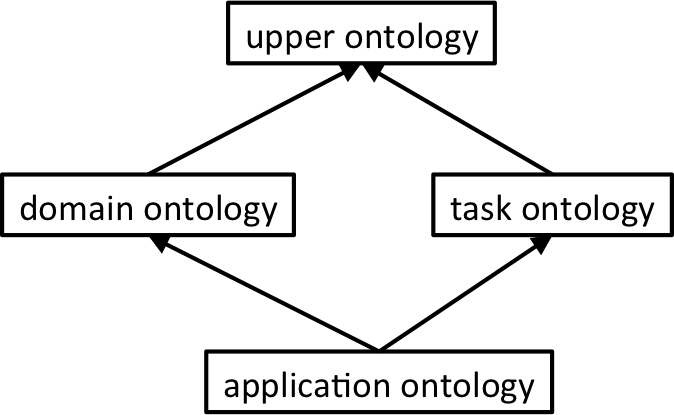
\includegraphics[width=0.5\textwidth]{ontologies-level-dependence.png}
%\caption[Types of ontologies according to level of dependence]{Types of ontologies according to level of dependence (Adapted from \cite{guarino1997semantic}).}
%\label{fig:ontologies-level-dependence}
%\end{center}
%\end{figure}

\subsubsection{Lightweight Ontologies and Heavyweight Ontologies}
\label{subsubsec:lightweight-ontologies}

%Based on the level of formal representation, ontologies can be classified in lightweight ontologies and heavyweight ontologies. As we can see in the Figure \ref{fig:spectrum-ontologies}, at one extreme, there are lightweight ontologies that consist of terms with little or no specification of the meaning. At the other end of the spectrum, we have heavyweight ontologies that comprise ontologies rigorously formalized by logical theories. As we move along the continuum, the amount of meaning specified and the degree of formality increases, reducing possible ambiguities \cite{uschold2004ontologies}.

%\begin{figure}[thbp]
%\begin{center}
%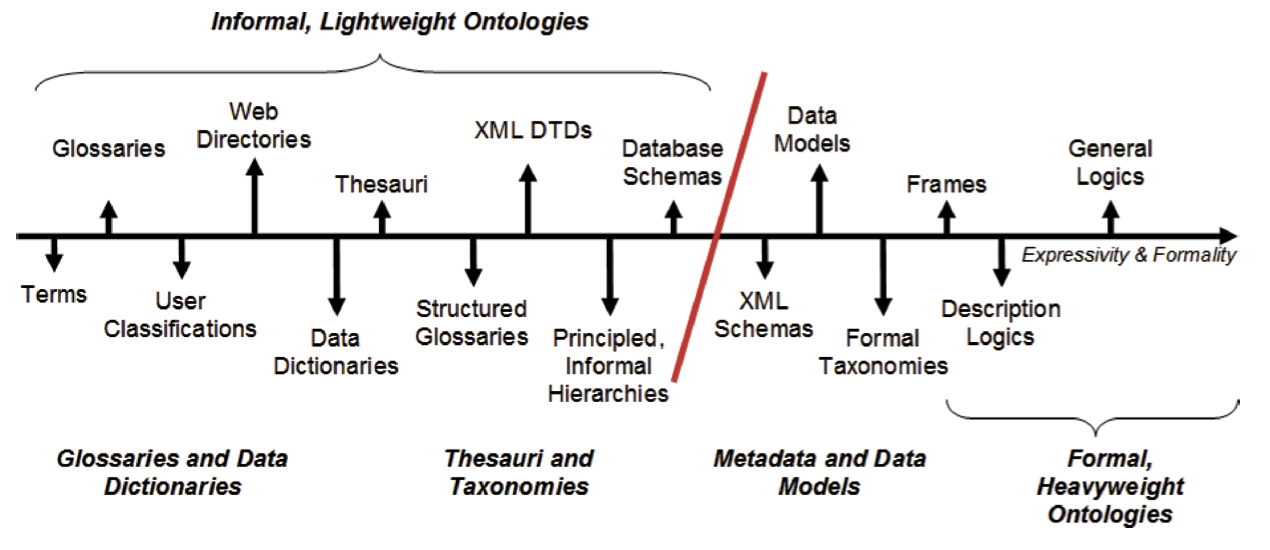
\includegraphics[width=0.85\textwidth]{spectrum-ontologies.png}
%\caption[The spectrum of lightweight and heavyweight ontologies]{The spectrum of lightweight and heavyweight ontologies (Taken from \cite{wong2012ontology}).}
%\label{fig:spectrum-ontologies}
%\end{center}
%\end{figure}

%The \emph{ligthweight ontologies} are ontologies based on topical hierarchies with lack rigorous conceptual definitions, principled conceptual organization, and label-concept distinctions. As instance of this kind of ontologies, we have terms, glossaries, thesauri, and database schemas. The main purpose of this kind of ontology is to provide a weak categorization of content to improve search engine functionality. Thus, the ligthweight ontologies are broadly used on the Web to categorize a large amount of data, such as available data on Web portals. However, these ontologies tend to be very usage-dependent and user-dependent of applications.

%The \emph{heavyweight ontologies} are much more than just lightweight ontologies. They are ontologies enriched with axioms for semantic interpretation of concepts and relations. Thus, the development of heavyweight ontologies needs a rigorous definition of concepts, an organization of defined concepts based on philosophical principles, a precise and formal semantic definition of relations among concepts, and so on. Heavyweight ontologies are important to create shareable and reusable knowledge bases, because they give more value to concepts represented on them by providing greater semantic precision and ensuring the fidelity and consistency of concepts about a target world.

%In this dissertation, we will develop the ontology OntoGaCLes as a heavyweight ontology, and application ontology for the domain of gamified CL scenarios.

\subsection{Ontology Representation}
\label{subsec:ontology-representation}

%Nowadays, the ontologies can be represented in two ways, one representation is the formal representation that is used for computer consumption, and another representation is the graphical representation for human comprehension. Both representations are relevant for this dissertation and they affect the quality of the representation of ontology.

\subsubsection{Formal Representation}
\label{subsubsec:formal-representation}

%To allow the formal representation for computer consumption, there are many languages that have been proposed using the predicate logics, description logics or frame based languages \cite{mizoguchi2004tutorial}. However, the most popular language and framework to describe ontologies is the Web Ontology Language (OWL) language that is based on the Resource Description Framework (RDF)/RDF-Schema.

%The RDF specification was developed by the World Wide Web Consortium (W3C) for metadata description. It is formally represented in the eXtensible Markup Language (XML) employing triplets that contain a subject node, predicate, and object node ($<$subject, predicate, object$>$). Each node in the triplet can be a web resource (URI reference), a value (literal) or a document identifier (to represent a blank node). A set of triples also can become a node itself, and a property is a semantic relation between nodes (subject and object).

%To represent triplets, the RDF/RDF-Schema specifications define classes, properties, and relationships that can be used to describe these triples as statements about resources. It also includes definition of tags and hierarchical structures (taxonomy) providing the basic elements for the description of ontologies. However, the RDF-Schema has some limitation, especially to support computational reasoning on data available through the internet \cite{patel2005building}. Thus, the OWL specification provides the expressive language to develop ontologies.

%OWL is a language developed and endorsed by the W3C to satisfy the formalism for the Semantic Web (SW). It allows the SW applications to understand and answer queries of agents (people or other programs) by reasoning on Web content by ontological descriptions. OWL was developed based on DAML+OIL \cite{horrocks2002damloil} with a formal specification influenced by description logics, the frames paradigms and the OWL exchange syntax (namely RDF/XML) \cite{horrocks2003shiq}.

%There are three variants of OWL referred as OWL Lite, OWL DL and OWL Full. These three variants allow to achieve a good balance between scalability and expressive power. According to the OWL specification, each variant is an extension of its simpler predecessor. Thus, OWL Lite is used manly for classification hierarchy and simple constraints; OWL DL gives maximum expressiveness retaining computational completeness and decidability; and OWL Full gives maximum expressiveness, however with no computational guarantees, the reasoning process using OWL Full may not be completed in a finite time. Figure \ref{fig:owl-example} shows as example part of an ontology related to bicycle in OWL.

%\begin{figure}[thbp]
%\begin{center}
%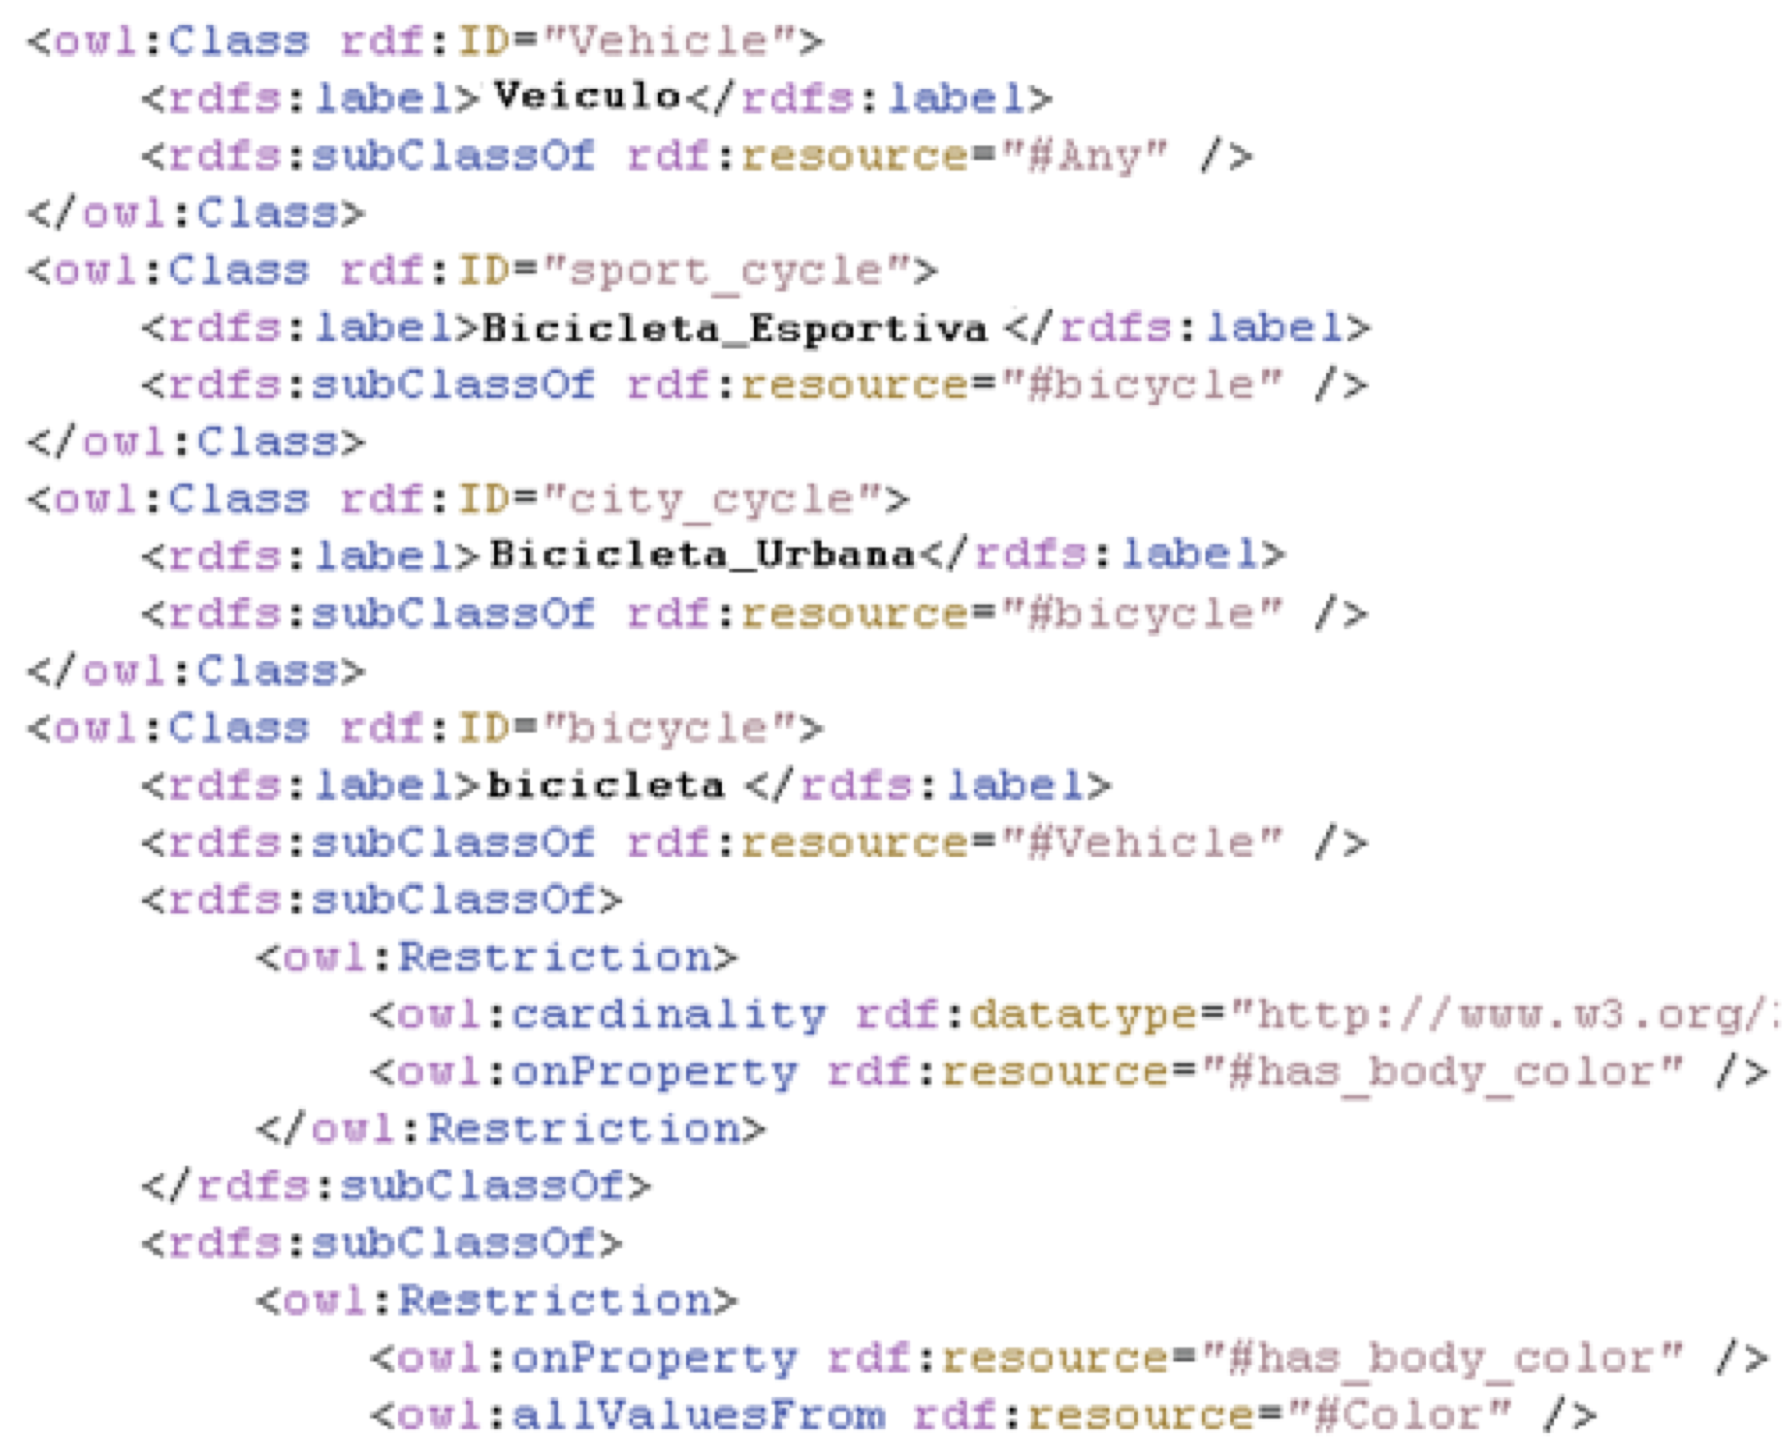
\includegraphics[width=0.65\textwidth]{owl-example.png}
%\caption[Part of bicycle ontology represented using OWL]{Part of bicycle ontology represented using OWL (Taken from \cite{isotani2010ontological}).}
%\label{fig:owl-example}
%\end{center}
%\end{figure}

%Since this dissertation will use graphical representation to describe the ontologies, we do not detail the RDF/RDF-Schema and OWL languages. RDF/RDF-Schema and OWL can be automatically generated by graphical ontology editors, such as Prot\'{e}g\'{e} \cite{noy2001creating}, OntoEdit \cite{sure2002ontoedit} and Hozo \cite{kozaki2002hozo}.

%\newpage
\subsubsection{Graphical representation}
\label{subsubsec:graphical-representation}

%Since an ontology is mainly composed by concepts and their relations, the graph is a common representation of ontologies, where the nodes represent concepts and the arrows represent relations between concepts \cite{dieng1998comparison}. Figure \ref{fig:graph-bicycle-ontology} shows an example of an ontology referred to bicycle. In this ontology, the concept of a bicycle is a specialization of vehicle represented using \emph{is-a} relation ($<$bicycle \emph{is-a} vehicle$>$). In ontology engineering, we can say that the class vehicle is a super-class of the class bicycle, and the bicycle is specialized into a sport bicycle and city bicycle. Finally, this Figure shows that the bicycle has attributes: color and weight. And the bicycle using the part-of relation is composed by elements: wheel, handlebar, frame and pedal. In this Figure, the scheme of colors helps the reader identify the relationship between concepts.

%\begin{figure}[thbp]
%\begin{center}
%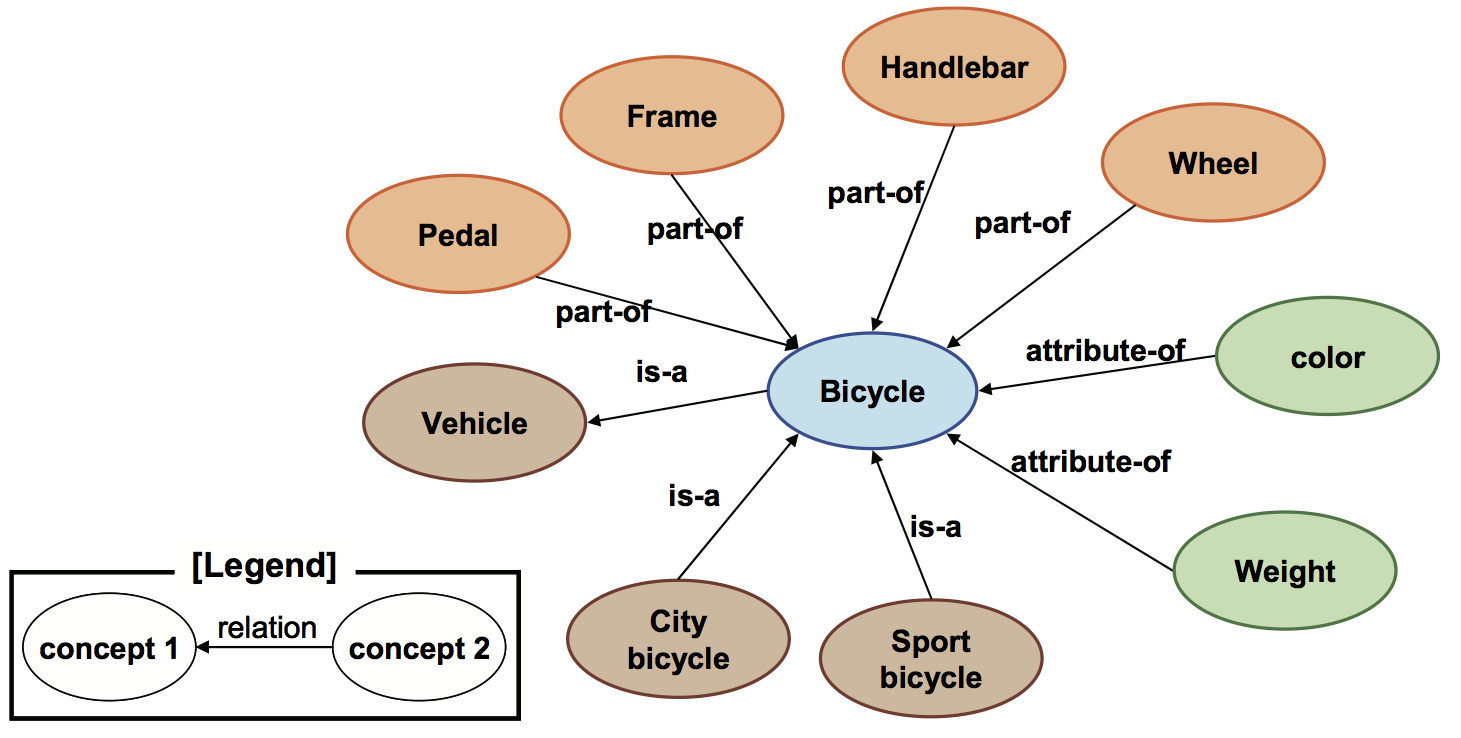
\includegraphics[width=0.8\textwidth]{graph-bicycle-ontology.png}
%\caption[A simple example of a bicycle ontology]{A simple example of a bicycle ontology (Taken from \cite{isotani2010ontological}).}
%\label{fig:graph-bicycle-ontology}
%\end{center}
%\end{figure}

%Although the representation of ontologies using graphs is the most common, it suffers deficiencies that do not help to capture important elements in an ontology \cite{devedzic2006semantic}, especially when trying to represent roles. Therefore, we decide to use the model of roles propose by \cite{ mizoguchi2007the}, and the Hozo ontology editor \cite{kozaki2002hozo} that is an authoring environment for building ontologies based on the model of roles.

%Hozo editor adequately deals with the differentiating of basic concepts (e.g. human, and artefact) from role concepts (e.g. learner, and reward) based on the model of roles. In this model, to deal with the concept of role, the following three classes are introduced: (a) Role concept - A concept representing a role that depends on a context (e.g. learner role that depends on the school); (b) Basic concept - A concept that does not need other concepts to be defined (e.g. human); and (c) Role holder - An instance of a base concept that is holding the role (e.g. learner). The basic concepts are used as class constraints, and the instances that satisfy the class constraints play the role, becoming role holders. For example as shown in the Figure \ref{fig:learner-role-hozo}, "In a learning environment there is a vacancy for a learner, and a person, whose name is Geiser, fills the position, becoming a learner in the particular environment." The person who plays a role is referred as a role holder. Thus, Geiser becomes a learner in the learning environment by playing the learner role. The top of the figure shows how the concepts around a role are related to each other and in the bottom is shown the representation in Hozo (without the instantiation of the person's name).

%\begin{figure}[thbp]
%\begin{center}
%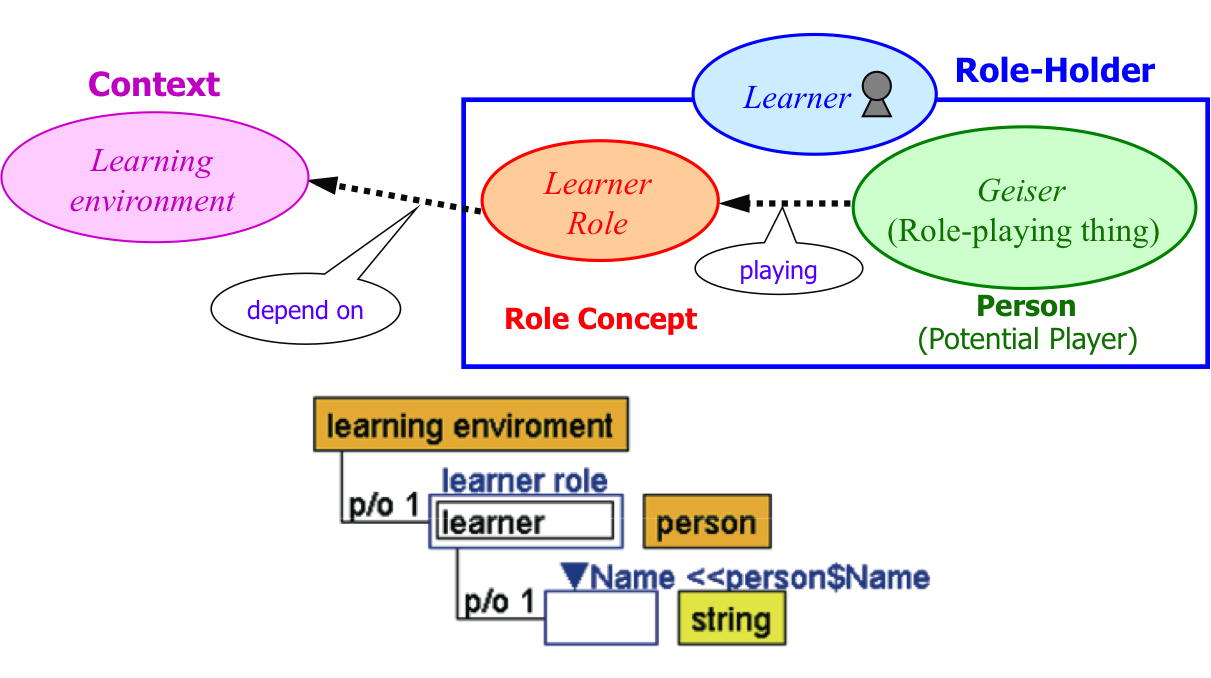
\includegraphics[width=0.65\textwidth]{learner-role-hozo.png}
%\caption[The learner role represented using Hozo]{The learner role represented using Hozo (Adapted from \cite{isotani2010ontological}).}
%\label{fig:learner-role-hozo}
%\end{center}
%\end{figure}

%Figure \ref{fig:hozo-bicycle-ontology} shows the representation of bicycle ontology using Hozo representation. In this figure, the relations part-of and attribute-of is respectively represented by labels "p/o" and "a/o" that appear in front of each slot. Thus, the frame, pedal, handlebar, and wheels are part of the bicycle. Observe that in the context of bicycle, a wheel (basic concept) can play the role of front wheel or rear wheel (role concepts). Thus, a particular instance of a wheel that plays one of these roles (front wheel role or rear wheel role) is referred to as role holder. In summary, a front wheel is an instance of wheel playing the front wheel role.

%\begin{figure}[thbp]
%\begin{center}
%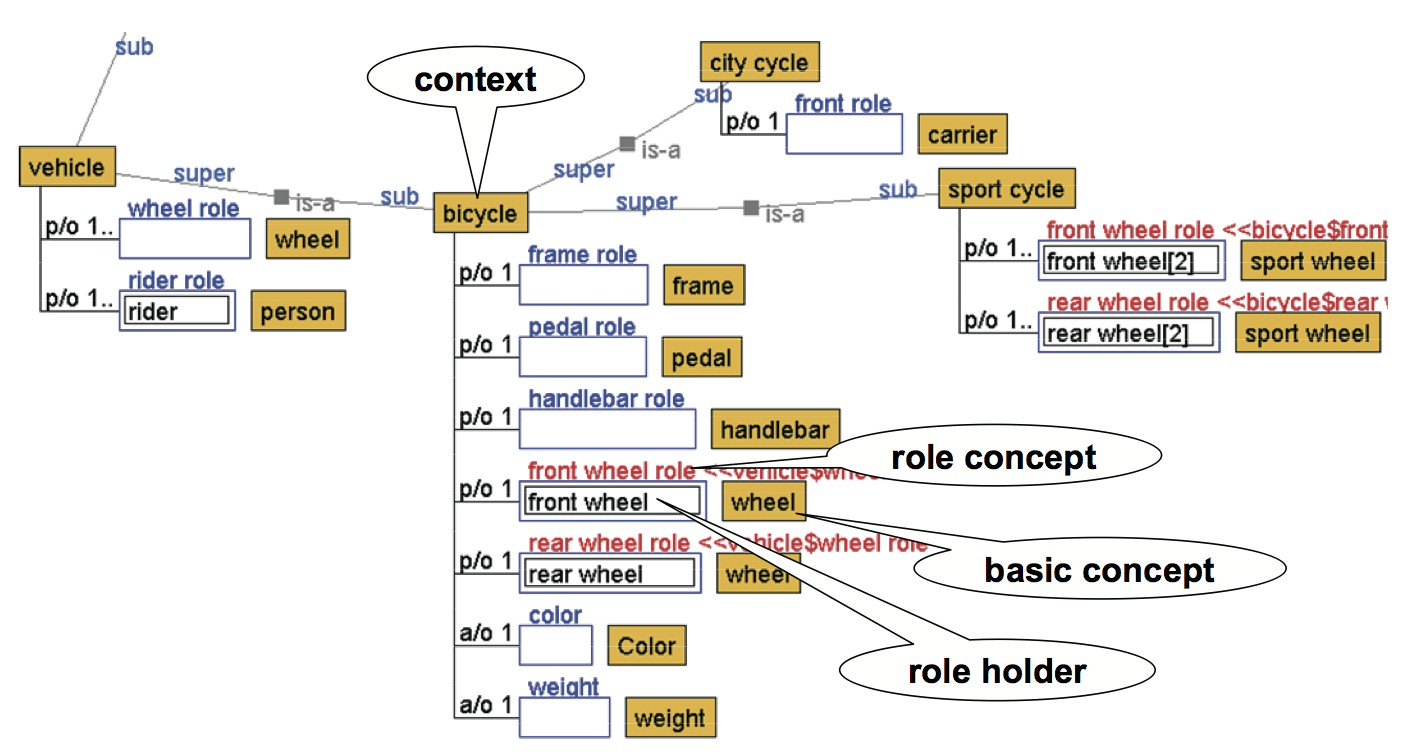
\includegraphics[width=0.95\textwidth]{hozo-bicycle-ontology.png}
%\caption[Example of bicycle ontology represented using Hozo]{Example of bicycle ontology represented using Hozo (Taken from \cite{isotani2010ontological}).}
%\label{fig:hozo-bicycle-ontology}
%\end{center}
%\end{figure}

\subsection{Ontology Engineering}
\label{subsec:ontology-engineering}

%According to \cite{devedzic2002understanding}, ontology engineering encompasses a set of activities conducted during the conceptualization, design, implementation and deployment of ontologies. It covers topics including philosophy, metaphysics, knowledge representation formalisms, development methodology, knowledge sharing and reuse, knowledge management, business process modeling, common sense knowledge, systematization of domain knowledge, information retrieval from the Internet, standardization, and evaluation.

%The development of ontologies is a time-consuming and difficult task that need knowledge about the target domain, theoretical background on otology research, and the skills to properly define the concepts and develop the body of knowledge. Thus, to facilitate the development of ontologies, there are several methodologies and methods for building ontologies. According to \cite{mizoguchi2004tutorial}, these methods are categorized into a three layer guideline as shown in Figure \ref{fig:three-layer-model}, in which:

%\begin{enumerate}
%\item \textbf{Top-layer} is the coarsest level which specifies the whole building process with standard software development life cycles. The ontological methodologies of top layer have a set of guidelines associated with conventional software development processes and practices.
%\item \textbf{Middle-layer} is the generic constraints and guidelines that specify a set of major steps and their order of execution. In each step of middle layer, the detailed information about the activities to be completed, and the way for each activity should be carried out. 
%\item \textbf{Bottom layer} is the most fine-grain guidelines that enable the construction of concepts hierarchy. It describes guidelines to create explicit semantic structures from identified concepts in the target world.
%\end{enumerate}

%\begin{figure}[thbp]
%\begin{center}
%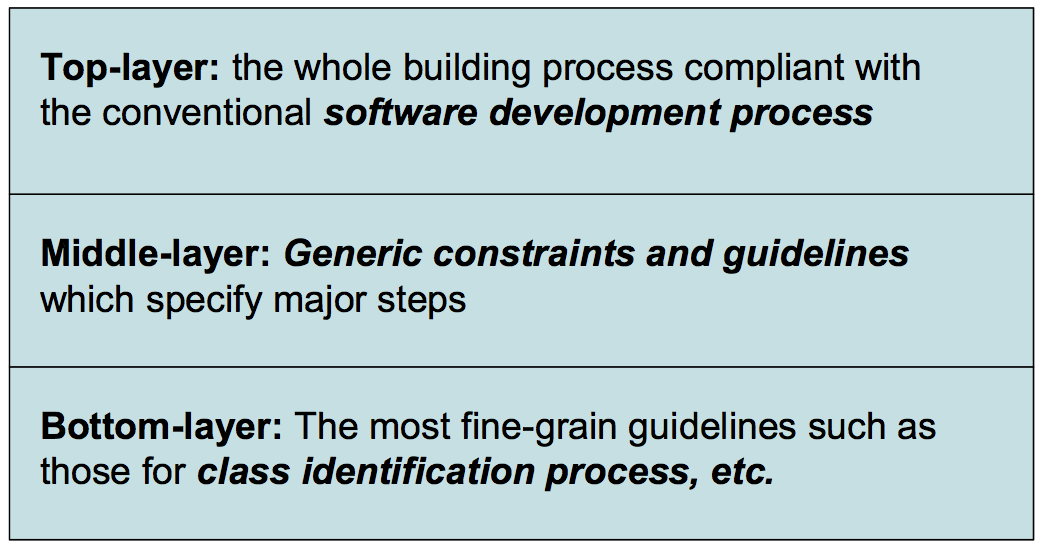
\includegraphics[width=0.75\textwidth]{three-layer-model.png}
%\caption[Three-layer model of ontology building methodology]{Three-layer model of ontology building methodology (Taken from \cite{mizoguchi2004tutorial}).}
%\label{fig:three-layer-model}
%\end{center}
%\end{figure}

%Most of the existing methodologies are concerned mainly with the top-layer. Some examples are METHONTOLOGY \cite{fernandez1997methontology}, On-To-Knowledge \cite{sure2004knowledge}, and Ushold and King’s methodology \cite{uschold1995towards}. Unfortunately, only a few methodologies deal with the middle and bottom layers.  The main problem of having few methodologies for the development of the middle and bottom layers is the lack of support for novices. Thus, the chances of creating a good ontology at the end of some process decreases condonably without guidelines for ontological development covering all the layers.

%In this sense, \cite{mizoguchi2004tutorial} offers guidelines to support the development of ontologies at the middle and bottom layers using the Activity-First Method for task ontology development \cite{mizoguchi1995ontology}. Thus, in this dissertation, we will utilizes these guidelines to create the ontology OntoGaCLeS. In the rest of this section, we present an overview of guidelines proposed by Mizoguchi in \cite{mizoguchi2004tutorial, mizoguchi2003part, mizoguchi2004part}.

%\subsubsection{Middle Layer Guidelines}
%\label{subsubsec:middle-layer}

%\begin{enumerate}
%\item Identify concepts rather than terms. As ontology is totally independent of terminological problems, one cannot stress the importance of this distinction too much. Since people will be easily trapped by the endless terminological discussion departing from the underlying conceptual structure of the target domain.
%\item Use mixed and flexible strategies of top-down, bottom-up and middle-out. Never stick to only one of the strategies. 
%\item Whenever possible, identify and use top-level ontology in the early phase of the development process to govern the rest of the steps. 
%\item When you deal with a concept, identify its main components, using “part-of” relation as well as its main attributes. You can thus find and extend candidates of concepts to be included in the ontology. 
%\item Definition of axioms should be done after finishing is-a hierarchy building and informal term definition. 
%\item Note that you cannot define any concept completely in theory. Therefore, do not stick to the definition of each term too much. At the best, you only can give necessary conditions of them. Term definition in the early phase can be rough. Detailed definition of a term should be done after you grasp the whole structure of the ontology, that is, after building is-a hierarchy. 
%\item Never try to seriously define a term one by one. Definition of a concept needs sufficient contextual information, which is usually not available in the early phase. Terms are related to each other and could have several meanings, which should be clarified by the context given. 
%\item Arrange and resolve the terminological issues(how to name a concept) at the last step. 

%\item When you find the necessity to define more than one meaning for one term, then you are facing the terminological problem. Each term should correspond to exactly one concept in ontology, since you are not building a dictionary, but a well-organized conceptual structure. Each term is only a label of the concept. You of course can build a dictionary after building ontology.

%\item Put a higher priority on is-a hierarchy construction than term definition. Carefully designed is-a hierarchy gives you a correct context to define a term.
%\item When you get stuck with a term definition, follow either one of the following : 
%\begin{itemize}
%\item Multiple meanings? Then concentrate on meaning one by one. 
%\item Multiple Viewpoints? Make the viewpoint explicit and then try it again 
%\item Check if you are discussing terminology.
%\item Use is-a hierarchy to give enough context. 
%\end{itemize}
%\end{enumerate}

\subsubsection{Bottom Layer Guidelines}
\label{subsubsec:bottom-layer}

%According to \cite{isotani2010ontological}, the following list summarizes the guidelines for the bottom layer:

%\begin{enumerate}
%\item \emph{Identify essential properties} for each concept considered essential in the scope of a given problem. These essential properties facilitate to create more stable concepts and hierarchies during the ontology development process.
%\item \emph{Make correct use of the role-concept} that can be defined as the association of a concept to a particular role within a given context. When developing an ontology, one should carefully distinguish the difference between role-concept, role-holder, and basic concepts. Such differentiation helps to treat multiple meanings as introduced previously in the guidelines for the Middle layer.
%\item \emph{Be careful when using is-a relation} in ontologies is different from the one utilized by object- oriented programming. The is-a relation applies only for classes. Furthermore, for given classes A and B the relation $<$class A is-a class B$>$ is true if and only if the instance set of A is a subset of the instance set of B. Therefore building a relation such as $<$teacher is-a human$>$ is ontologically incorrect, since \emph{teacher} is not an ontologically-valid class because there is no person (no instance of class person) whose intrinsic property is being a teacher. Thus, in ontology, it is inappropriate to model $<$Mizoguchi instance-of Teacher$>$ and $<$Teacher is-a Human$>$ (What happens if Mizoguchi quits his job?).
%\item \emph{Be careful when using part-of relation} such as functional, qualification, spatial and etc. Thus, it needs to be used carefully, especially avoid part-of relation to create class hierarchies such as $<$man part-of human$>$. Such an expression is valid only when you want to deal with man as a subspecies of human.
%\item \emph{Pay attention to the difference between is-a and part-of relations}. Usually, the meaning of is-a and part-of relations is easy to distinguish. The former indicates generic vs. specific relations between classes. The latter is often utilized to specify the composition of a thing (although, part-of can be used in other situations). However, sometimes when developing an ontology, one can encounter difficulties to distinguish their difference. For example, which of the following relation is correct: $<$Dog part-of mammal living in Japan$>$ or $<$Dog is-a mammal living in Japan$>$? People agree that $<$Dog is-a mammal$>$ is correct. However, by adding the \emph{living in Japan} phrase to mammal the distinction is not quite that easy because \emph{mammal living in Japan} seems to represent species, and therefore, $<$\emph{dog-species} part-of  \emph{mammal-species} living in Japan$>$ could be considered. Thus, the distinction between is-a and part-of relation is not always easy.
%\item \emph{Avoid the use of multiple inheritances} Creating multiple inheritances is the source of many problems to keep the consistency of the representation. In particular, propagating the essential properties is a problem since each concept should be recognized and represented by their own essential properties.
%\item \emph{Some boundary between similar concepts can be vague} When developing an ontology some boundaries between similar concepts do not need to be strongly conceptualized. An example is the distinction between the concepts black and white. Since the distinction between them is based on the ambiguous color gray, we cannot give a clear and unique boundary between black and white (although we recognize their existence).
%\item \emph{Create terms if there is no label to represent a concept}. If you cannot find an appropriate term to represent a concept, then you can temporarily label them with some sentences or marks (e.g., concept 1 and concept 2) until you can come up with a good label. When the body of the ontology is good enough to represent the target domain, you can revise the labels of each concept.
%\end{enumerate}





